\chapter{Introduction}
Wikipedia is the biggest source of information currently available on the Internet, there are more
than 6 million articles in the English Wikipedia and they are all maintained by volunteers. The
value of Wikipedia is all in the editors' hands.

Thousands of users edit Wikipedia everyday. Many users means many different ideas and therefore an
higher probability of a disagreement; this means there are conflicts are on the agenda. Avoiding or
reducig these conflicts is the best way for this encyclopedia to grow. \\

Each Wikipedia page has four different tabs:  
\begin{itemize}
    \item Article: the actual content of the page.
    \item Talk Page: a forum where people can talk about edits. 
    \item History: a place where everyone can see the older versions of the pages.
    \item Source: a section where users can edit the page. 
\end{itemize}

Conflicts could happen both on the Talk page, through a discussion, and in the Article, through an
edit war. It is valuable to analyze all these aspects to get a well-rounded view of the problem.

\begin{figure}
    \centering
    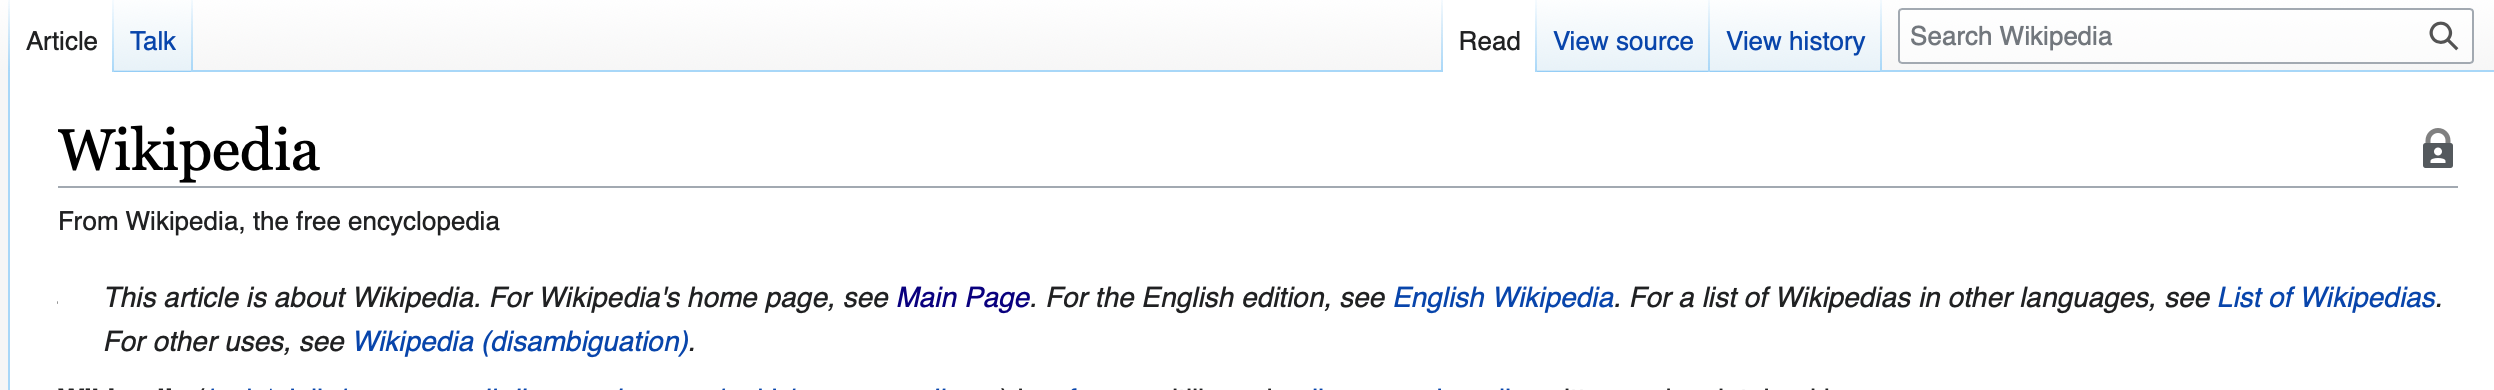
\includegraphics[width=1\textwidth]{./chapters/01/assets/wikipedia_page.png}
    \caption{Page structure.}
    \label{fig:page}
\end{figure}

\section{Main Project}
\label{sec:Main Project}
The project our team, in collaboration with Eurecat and the Wikimedia Foundation, is working on
is called: “Community Health Metrics: Understanding Editor Drop-off“. This is an excerpt of the
project idea: \\

“The primary value of Wikipedia is the editors. When an editor leaves the project, we lose their
participation and contribution to the community, This could be related to multiple factors, also
external to the project, but it could signal an issue related to internal dynamics and to the health
of the community. While a big effort was dedicated to retain new editors, we lack knowledge and
initiatives focused on understanding and preventing drop-off for experienced editors.”
\\
As stated in the project description, the focus is on expert users, who are the core of Wikipedia:
there are 41,741,926 Wikipedia accounts but only 132,916 users are active, nearly 3\% of all
users\footnote{\url{https://stats.wikimedia.org/EN/TablesWikipediansEditsGt5.htm}}. 

Focusing on this category of users and understanding the reasons that lead to a drop-off can give Wikipedia a
big help. Several people are working on this project, because it's just a part of the whole.
In the team, everyone is working on a specific topic with the idea of then merging the different
results to obtain an analysis of the phenomenon from different points of view in order to have a
better understanding of the life cycle of users.  

The prevention of the drop-off is not the only goal of the project, improving the community health
is also important to let users be in a good environment without being held back from editing. 

\section{My Contribution}
\label{sec:project}
The topic explored in this study is the revert analysis - i.e., when the version of a page is
restored to that of a specific date - for all the articles of Wikipedia.

This project consisted in the analysis of the edit history of different language editions of
Wikipedia to study patterns of reverts and edit wars to understand their potential effect on
individual user activity.

We implemented state-of-the-art metrics of controversy based on reverts and mutual reverts and
developed a new metric based on revert chains. Metrics have been computed per page and per user
monthly.



\section{Related Work}
There are several works involving reverts: An interesting tool that allows visualizing conflicts is
the one developed by Suh \textit{et al.}~\cite{Suh2007}. The problem is that it is from 2007 but
Wikipedia started to grow a lot since then; now we have new technologies and much more data to
analyze therefore more interesting conclusions can be reached. There have been analysis of antisocial
behavior caused by vandalism~\cite{Kiesel2017}, but since the focus of the project is on experienced
users, this is not relevant to this study. In 2014 Yasseri \textit{et al.}\cite{Yasseri2014}
defined a controversy metric based on mutual reverts, called M. In this study we used this metric as a starting
point to develop another controversy metric based on reverts chains, called G. We computed metrics for both
page and users including M.